% SC4063 --- Chapter 7: Monitoring, Forensics and Zero Trust (0->100)
\chapter{Monitoring, Forensics and Zero Trust}\label{ch:monitor}
\sloppy

\begin{quote}
\emph{``You cannot hunt what you never collected.''} --- Detection starts before the incident, in the quiet decision to keep the right logs and to distrust the network you already own.
\end{quote}

\noindent\fbox{\parbox{\dimexpr\linewidth-2\fboxsep-2\fboxrule}{%
\textbf{From zero: seeing, trapping, and trusting nothing.} We start from a mirrored packet, compress it into a flow, store it for a hunt, lure the attacker into a fake service, and finally stop trusting the wire at all. Intuition (pipe $\to$ tap) $\to$ collection $\to$ deception $\to$ zero trust. No prior SOC background assumed.}}
\vspace{0.4em}

\section*{Learning Outcomes}
After this chapter you will be able to:
\begin{enumerate}[label=(L\arabic*)]
    \item capture and dissect traffic with \texttt{tcpdump}/Wireshark and summarise it as NetFlow/IPFIX;
    \item deploy honeypots/honeynets and DNS/BGP hardening (DNSSEC, RPKI) as network sensors;
    \item run a forensics workflow: preserve $\to$ timeline $\to$ IoC hunt $\to$ attribute;
    \item query a SIEM (Splunk SPL) and build visibility baselines for alerting;
    \item contrast perimeter (castle-moat) with zero trust (NIST 800-207) and map to ZTNA.
\end{enumerate}

% ============================================================
\section{Seeing the Wire: Capture to SIEM}\label{sec:visibility}
A tap copies light (passive, no latency); a SPAN/mirror copies in the switch ASIC (cheap, may drop under load). Either feeds capture.

\texttt{tcpdump} (CLI, \texttt{libpcap}) and Wireshark (\texttt{pyshark}) dissect the copy; NetFlow/IPFIX summarise it. A flow is the 5-tuple plus counters: bytes, packets, start, duration, flags. Collectors (e.g., \texttt{nfdump}, \texttt{pmacct}) export flows to a SIEM, which correlates IDS alerts, flows, and host logs on one timeline. Sampling (1:100) is required at 10\,Gbps.

\begin{figure}[h]\centering
\resizebox{\linewidth}{!}{%
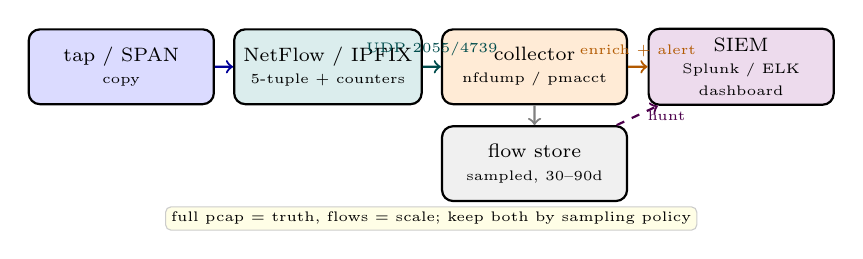
\begin{tikzpicture}[scale=0.82, every node/.style={font=\scriptsize},
  mybox/.style={draw,thick,rounded corners=4pt,minimum width=2.35cm,minimum height=0.95cm,align=center}]
\node[mybox,fill=blue!14] (tap) at (0,1.65) {tap / SPAN\\\tiny copy};
\node[mybox,fill=teal!14] (flow) at (3.2,1.65) {NetFlow / IPFIX\\\tiny 5-tuple + counters};
\node[mybox,fill=orange!16] (coll) at (6.4,1.65) {collector\\\tiny nfdump / pmacct};
\node[mybox,fill=violet!14] (siem) at (9.6,1.65) {SIEM\\\tiny Splunk / ELK\\\tiny dashboard};
\node[mybox,fill=gray!12] (store) at (6.4,0.15) {flow store\\\tiny sampled, 30--90d};
\draw[->,thick,blue!60!black] (tap) -- (flow);
\draw[->,thick,teal!60!black] (flow) -- (coll) node[midway,above,font=\tiny] {UDP 2055/4739};
\draw[->,thick,orange!70!black] (coll) -- (siem) node[midway,above,font=\tiny] {enrich + alert};
\draw[->,thick,gray] (coll) -- (store);
\draw[->,thick,dashed,violet!60!black] (store) -- (siem) node[midway,right,font=\tiny] {hunt};
\node[font=\tiny,fill=yellow!10,rounded corners=2pt,inner sep=2pt,draw=gray!40] at (4.8,-0.70) {full pcap = truth, flows = scale; keep both by sampling policy};
\end{tikzpicture}}%
\caption{Visibility pipeline. A passive copy becomes flows at the collector and incidents in the SIEM. Sampling and retention policy determine what you can hunt tomorrow.}
\label{fig:visibility}
\end{figure}

Baselining turns collection into detection: per-subnet bytes, per-service entropy, and per-host outbound flows per hour. A host that normally opens 30 flows/hour and suddenly opens 2\,000 to port~443 on many destinations is beaconing until proven otherwise.

\begin{lstlisting}[language=bash,caption={From packet to flow to hunt: tcpdump, nfdump, and Splunk SPL.},label={lst:flow}]
# Capture: 60s of DNS and SYN on the DMZ mirror
tcpdump -i eth1 -w dmz.pcap -G 60 -W 1 'port 53 or tcp[tcpflags] & tcp-syn != 0'
# NetFlow: synthesise flows from the pcap, then top talkers
nfdump -r dmz.nf -o extended -s ip/bytes -n 10   # top 10 by bytes
nfdump -r dmz.nf 'port 53' -o csv | head          # DNS flows for hunting
# Splunk SPL: beaconing and DNS tunnelling intuition
# | tstats count where index=netflow by src_ip, dst_ip
# | where count > 1000 | sort -count
# search index=dns query_length > 80 | stats count by src_ip | where count > 200
\end{lstlisting}

% Python aggregation moved to text: top talker via Counter, beacon via threshold -- see runbook for full script.

% ============================================================
\section{Deception and Hardened Naming/Routing}\label{sec:honeypot}
A honeypot is a fake vulnerability that is cheap for you and expensive for the attacker to verify. Low-interaction (e.g., \texttt{cowrie} SSH) emulates a service; high-interaction runs a real instrumented host. A honeynet is a subnet of honeypots with a darknet (unused address space) around them. Any packet there is suspicious by construction; an alert from the honeynet has far higher precision than one from production.

\begin{figure}[h]\centering
\resizebox{\linewidth}{!}{%
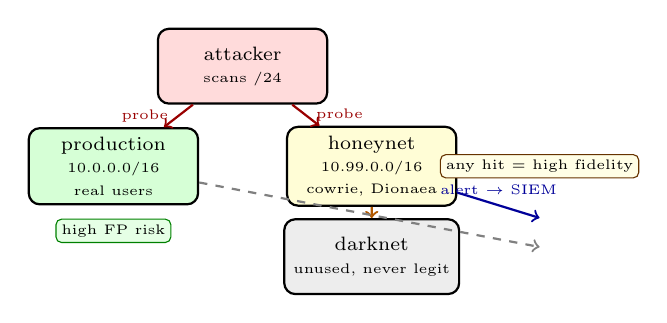
\begin{tikzpicture}[scale=0.82, every node/.style={font=\scriptsize},
  net/.style={draw,thick,rounded corners=4pt,minimum width=2.15cm,minimum height=0.95cm,align=center}]
\node[net,fill=green!16] (prod) at (0,1.65) {production\\\tiny 10.0.0.0/16\\\tiny real users};
\node[net,fill=yellow!16] (honey) at (4.0,1.65) {honeynet\\\tiny 10.99.0.0/16\\\tiny cowrie, Dionaea};
\node[net,fill=gray!14] (dark) at (4.0,0.25) {darknet\\\tiny unused, never legit};
\node[net,fill=red!14] (atk) at (2.0,3.20) {attacker\\\tiny scans /24};
\draw[->,thick,red!60!black] (atk) -- (prod) node[midway,left,font=\tiny] {probe};
\draw[->,thick,red!60!black] (atk) -- (honey) node[midway,right,font=\tiny] {probe};
\draw[->,thick,orange!70!black,dashed] (honey) -- (dark);
\node[font=\tiny,fill=green!10,rounded corners=2pt,inner sep=2pt,draw=green!50!black] at (0,0.65) {high FP risk};
\node[font=\tiny,fill=yellow!10,rounded corners=2pt,inner sep=2pt,draw=orange!40!black] at (6.6,1.65) {any hit = high fidelity};
\draw[->,thick,blue!60!black] (honey) -- (6.6,0.85) node[midway,above,font=\tiny] {alert $\to$ SIEM};
\draw[->,thick,gray,dashed] (prod) -- (6.6,0.40);
\end{tikzpicture}}%
\caption{Honeypot vs.\ production. Production alerts are noisy; a darknet/honeynet has no legitimate traffic, so any contact is an attacker to investigate. Logs feed the same SIEM with higher priority.}
\label{fig:honeypot}
\end{figure}

DNS and BGP are network infrastructure worth hardening as sensors. DNSSEC signs zones (RRSIG/DNSKEY) so resolvers can validate answers and detect cache poisoning; RPKI signs BGP route origins (ROA) so routers can reject hijacks. Neither encrypts, but both make spoofing detectable and therefore huntable.

\begin{lstlisting}[language=bash,caption={Low-interaction honeypot and DNS/BGP validation checks.},label={lst:cowrie}]
# Cowrie SSH honeypot (low interaction, JSON logs to SIEM)
pip install cowrie && cowrie start --listen 0.0.0.0:2222
tail -f ~/cowrie/var/log/cowrie/cowrie.json | jq '.eventid, .src_ip, .input'
# DNSSEC validation check
dig +dnssec example.com | grep -i "ad flag"   # AD=1 means validated
delv @8.8.8.8 example.com                      # verbose DNSSEC chain
# RPKI origin validation (routinator / rpki-client)
rpki-client -v && bgpq3 -b -4 AS13335         # fetch ROAs, build prefix filter
\end{lstlisting}

Preserve forensics discipline: image with \texttt{dd} plus hash, freeze clocks (NTP), and keep a chain of custody. Then build a timeline (\texttt{plaso/log2timeline}, Zeek logs, auth logs), hunt IoCs (hashes, JA3, beacon intervals), and attribute with care: infrastructure is cheap to rotate, TTPs are harder to fake.

% ============================================================

\section{Forensics: Preserve, Timeline, Hunt}\label{sec:forensics}
Forensics is not incident response; it is the evidence discipline that makes response defensible. \emph{Preserve} means bit-for-bit imaging (\texttt{dd if=/dev/sda | sha256sum}), freezing clocks, and chain-of-custody notes: who collected, when, hash. Volatility or \texttt{LiME} captures RAM before it is lost. Write-blockers prevent the investigator from becoming the attacker.

\emph{Timeline} merges sources on one clock: Zeek \texttt{conn.log} (every flow), \texttt{auth.log} (every login), EDR process trees, and firewall allows. \texttt{plaso} (\texttt{log2timeline}) normalises timestamps; even one skewed host (NTP off by minutes) creates false causality. Hunt next: pivot on IoCs (hash, IP, JA3, domain) across the timeline, not just in one log. A single beacon at 3\,a.m.\ to a new AS is interesting; three such beacons spaced exactly 300\,s apart is attribution-grade.

\begin{remark}[Attribution caution]\label{rem:attr}
Infrastructure is cheap to rotate; TTPs are not. An IP that was the C\&C last week may be a compromised home router today. Correlate TTPs (beacon interval, User-Agent, DNS pattern) plus human context before naming an actor. False attribution is a second incident.
\end{remark}

A minimal hunt query: start from a honeynet hit, extract its source IP and JA3, search NetFlow for prior flows with the same JA3, then check which production host contacted that IP before the honeynet did. That host is patient zero until proven otherwise.

\section{Zero Trust: From Castle-Moat to Mesh}\label{sec:zerotrust}
A perimeter assumes inside is safe; compromise of one host then grants lateral movement. Zero trust (NIST SP~800-207) assumes the network is hostile and checks every flow as if it crossed the Internet: authenticate the user and device, authorise per resource, encrypt per flow, and log centrally. The enterprise becomes a set of micro-perimeters around each service, with a policy engine that grants short-lived access.

\begin{figure}[h]\centering
\resizebox{\linewidth}{!}{%
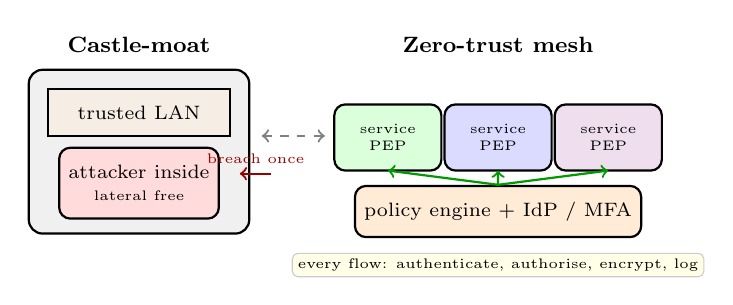
\begin{tikzpicture}[scale=0.80, every node/.style={font=\scriptsize},
  box/.style={draw,thick,rounded corners=4pt,minimum width=1.95cm,minimum height=0.90cm,align=center}]
% castle
\node[font=\footnotesize\bfseries] at (1.6,3.15) {Castle-moat};
\draw[thick,fill=gray!12,rounded corners=5pt] (-0.15,2.75) rectangle (3.35,0.15);
\draw[thick,fill=brown!14] (0.15,2.45) rectangle (3.05,1.70) node[midway] {trusted LAN};
\node[box,fill=red!14] (atk1) at (1.6,0.95) {attacker inside\\\tiny lateral free};
\draw[->,thick,red!60!black] (3.70,1.10) -- (3.20,1.10) node[midway,above,font=\tiny] {breach once};
% mesh
\node[font=\footnotesize\bfseries] at (7.3,3.15) {Zero-trust mesh};
\foreach \x/\y/\col in {5.55/1.70/green!14,7.30/1.70/blue!14,9.05/1.70/violet!13} {
  \draw[thick,fill=\col,rounded corners=4pt] (\x-0.85,2.20) rectangle (\x+0.85,1.15) node[midway,align=center,font=\tiny] {service\\PEP};
}
\node[draw,thick,fill=orange!16,rounded corners=4pt,minimum width=3.4cm,minimum height=0.65cm] (pe) at (7.30,0.50) {policy engine + IdP / MFA};
\foreach \x in {5.55,7.30,9.05} {\draw[->,thick,green!60!black] (pe.north) -- (\x,1.15);}
\node[font=\tiny,fill=yellow!10,rounded corners=2pt,inner sep=2pt,draw=gray!40] at (7.30,-0.35) {every flow: authenticate, authorise, encrypt, log};
\draw[<->,thick,dashed,gray] (3.55,1.70) -- (4.55,1.70);
\end{tikzpicture}}%
\caption{Perimeter vs.\ zero trust. The castle trusts by location; the mesh trusts by identity and checks per flow at a Policy Enforcement Point. Breach blast radius shrinks from the whole LAN to one resource.}
\label{fig:zerotrust}
\end{figure}

NIST 800-207 components: Policy Engine (decides), Policy Administrator (provisions), Policy Enforcement Point (PEP, enforces on the data path), plus IdP, device inventory, and continuous diagnostics. ZTNA replaces VPN's coarse ``inside'' with per-app tunnels (often WireGuard or mTLS) and removes standing privilege: access expires in minutes, not months. Migration is incremental: identify crown jewels, put a PEP in front, require MFA and device posture, then expand the mesh.

% ============================================================

Migration is four incremental cuts, not a flag day. (1) Inventory: list every service, data store, and current trust boundary. (2) Crown jewels first: put a PEP in front of the DB and require MFA plus device posture. (3) Expand the mesh service by service; each cut adds one PEP and one policy, old VPN routes are pruned. (4) Continuous verification: device health, user risk, and flow baselines feed the policy engine; a compromised device loses access in minutes, not at the next password rotation.

ZTNA tunnels are often WireGuard or mTLS per app, not one flat network. A user who can reach the wiki should not automatically reach the build system. Micro-segmentation is the network realisation of least privilege from Ch.~2, now enforced per flow rather than per VLAN.

\section{Exercises}\label{sec:ch07-exercises}
\begin{enumerate}[label=E7.\arabic*, leftmargin=*, itemsep=0.6em]
    \item \textbf{Baseline.} From one hour of NetFlow for \texttt{10.0.0.0/16}, compute per-host flows/hour and bytes/flow. Flag a host that jumps from 30 to 2\,000 flows/hour to many /24s. What alert threshold would you set to keep false positives $<5\%$?
    \item \textbf{Honeypot triage.} A cowrie log shows \texttt{root/admin} logins from \texttt{203.0.113.77} trying \texttt{wget http://203.0.113.77/mips}. Is this automated? List three IoCs to hunt in SIEM and one action to block the follow-on.
    \item \textbf{DNSSEC/RPKI.} A resolver without DNSSEC sees a poisoned A record; one with DNSSEC sees it. Explain the validation that fails (RRSIG) and similarly how an RPKI-invalid BGP announcement is distinguished from a legitimate one.
    \item \textbf{Forensics timeline.} A host was compromised at $T_0$. You have Zeek \texttt{conn.log}, auth.log, and cowrie hits. Sketch preserve$\to$timeline$\to$IoC$\to$attribute for the first 30 minutes and name the artefact that proves lateral movement vs.\ inbound scan.
    \item \textbf{Zero trust map.} Map a VPN-based remote access (castle-moat) to NIST 800-207: where are the PE, PA, and PEP, and what changes when you replace it with ZTNA per-app tunnels? Name one usability win and one deployment pitfall.
\end{enumerate}

\begin{remark}[Operational note]\label{rem:opnote}
This design assumes continuous tuning, not a one-time deploy. Thresholds drift with traffic growth; retrain baselines monthly and after any architecture change. A threshold that was correct at 1\,Gbps is noise at 10\,Gbps.
Log retention is a cost decision: 30\,days of full NetFlow at 10\,Gbps sampled 1:100 is $\approx$2\,TB; justify it against the forensics window your IR team needs. Keep honeynet logs longer because they are tiny and high value.
Every automation (auto-block, auto-quarantine) needs a manual override and an audit trail. An auto-block that triggers on a CDN PoP will outage your own users; require a second signal (e.g., honeynet + NetFlow) before blocking a /24.
\end{remark}
Retention is policy, not storage: 90\,days of sampled NetFlow at 1:100 on a 10\,Gbps link is roughly 2\,TB with compression, while full pcap for the same window is petabytes. Keep full pcap for the last 72\,h on a ring buffer and flows for 90\,days; justify the window against your mean time to detect.
Normalize before you correlate: \texttt{log2timeline} plus Zeek and EDR timestamps must share NTP. A host whose clock drifts by 2\,minutes will appear to beacon after the C\&C was blocked, inverting causality. Alert on NTP skew as a sensor health check.
Honeynet fidelity comes from isolation: the honeynet VLAN must have no route to production and no legitimate user should ever learn its address. Any hit is then high priority by construction. Mirror the same SIEM rules but with lower thresholds for the honeynet and page on first hit.
DNSSEC and RPKI are validation, not encryption: DNSSEC proves the answer was not tampered, RPKI proves the BGP origin is authorized. Both fail closed only if you enforce validation; otherwise they are merely observable. Log validation failures and alert on RPKI-invalid or DNSSEC-bogus at the resolver.
Baseline per VLAN, not globally: a DMZ web server that normally serves 10\,k flows/hour looks different from a management jump host that serves 20. Per-VLAN baselines reduce false positives and let a 5\,flows/hour beacon stand out on a quiet host.
Splunk cost control: index only what you hunt. Drop debug logs, sample health checks, and keep honeypot JSON at full fidelity. A SIEM that is 90\% noise will be ignored; a SIEM that is 10\% honeynet and baseline breaches will be watched.
Zero-trust rollout needs a fallback: when the policy engine is unreachable, fail closed for crown jewels and fail open with alerting for low-value wikis. Document the fallback per PEP and test it by killing the PA during a tabletop.
Device posture is the unsung control: a PEP that checks MFA but not patch level will grant a compromised laptop the same access as a clean one. Integrate EDR health into the policy engine and revoke short-lived certs when health drops.
Tune thresholds after every major release: a new video endpoint that streams 10\,MB per request will shift the per-host bytes baseline and create false positives if the SIEM still uses the old mean.
Tag flows with business context: ``prod-web'', ``guest-wifi'', ``build''. A spike tagged ``guest-wifi'' at 2\,a.m.\ is less urgent than the same spike on ``prod-db''; context prevents alert fatigue.
Keep the darknet small but representative: a /24 darknet inside a /16 is enough to see scans without consuming address space. Route it to the honeynet collector and alert on any SYN to it.
Test DNSSEC validation in staging: a misconfigured trust anchor will mark legitimate domains as bogus and break resolution. Monitor \texttt{SERVFAIL} rate after enabling validation and have a rollback key.
RPKI ROA expiry is an outage: if your ROA expires, peers that validate will drop your prefix. Automate ROA renewal and alert 30\,days before expiry; keep a non-validating peer for emergency reachability.
Use JA3 and JA3S for TLS fingerprinting, but remember they are brittle: a client update changes the fingerprint. Combine JA3 with destination and timing, not alone, to avoid false attribution.
Sampling must be consistent across collectors: if one router samples 1:100 and another 1:1000, top-talker comparison is meaningless. Standardise sampling and annotate it in every dashboard.
Encrypt log transport: NetFlow and syslog over UDP are trivial to spoof. Use TLS-wrapped export (IPFIX over TLS) or at least HMAC the feed; otherwise an attacker can inject fake flows to distract the SOC.
Practice evidence preservation under pressure: have a one-page checklist (image, hash, chain of custody) laminated at the jump host. During an incident, people skip steps unless the checklist is physical.
Rotate honeypot credentials weekly: if the honeypot always uses \texttt{admin:password}, attackers learn to ignore it. Use realistic but fake credentials and monitor which ones are tried first.
Correlate across time windows: a beacon every 300\,s will be missed by a 60\,s window but caught by a 10\,minute autocorrelation. Use both short and long windows in the SIEM.
Document data sources per alert: ``this alert fired because NetFlow + Suricata SID 1000001 + honeynet hit'' is actionable; ``anomaly score high'' is not. Provenance builds trust in the SIEM.
Limit honeynet outbound: a high-interaction honeypot that is allowed to attack others becomes liability. Rate-limit and sinkhole outbound from the honeynet at the hypervisor.
Baseline DNS query length and qtype distribution: DNS tunnelling uses long TXT or NULL queries. A host that normally queries A/AAAA and suddenly queries 80-char TXT is exfiltrating until proven otherwise.
Keep a canary token in the honeynet: a fake AWS key or cookie that, when used, triggers an alert. Its use proves the attacker exfiltrated and tried to reuse, not just scanned.
Integrate threat intel as context, not as blocklist: an IoC that is two weeks old is likely reassigned. Use intel to pivot hunts, not to auto-block, unless freshness is proven.
Score alerts by precision: honeynet = 0.99, NetFlow baseline breach = 0.30, IDS signature = 0.70. Route high-precision alerts to paging, low-precision to a queue reviewed daily. Precision determines on-call load.
For forensics, capture process trees, not just flows: a host that contacts a C\&C and then spawns \texttt{powershell} is compromised; a host that merely contacts it may be a browser misfire. EDR context disambiguates.
Zero-trust policy needs negative testing: try to reach a service you should not reach and prove the PEP blocks. A policy that is never tested for denial is a policy that may be misconfigured to allow.
Archive SIEM rules with the policy: when a rule is tuned or disabled, record who, why, and the expected false-positive reduction. Untuned rules are re-enabled by accident and flood the SOC again.
Measure hunt success: track mean time to detect, mean time to triage, and fraction of alerts that were true positives. Improve the worst metric each quarter, not all at once.
Finally, rehearse the forensics handover: a junior analyst should be able to take a preserved image and rebuild the timeline from runbook alone. If the handover needs the original analyst, the documentation failed.
Continuous learning closes the loop: every incident's IoCs become tomorrow's SIEM rules, and every false positive becomes a tuned threshold. The SIEM is a living system, not a deploy-once product.
Continuously validate NTP across the fleet: a host that drifts will break forensic timeline reconstruction; alert when offset exceeds 500\,ms and auto-correct via chrony.
Tune honeynet alert routing: page the SOC immediately on any honeynet hit, but batch NetFlow baseline breaches into a daily digest to avoid paging fatigue.
Document the RPKI fallback: if the validator is down, do not fail closed on all BGP; keep one non-validating session for emergency reachability and log the exception.
Use canary files on production hosts: a file that should never be read; its access triggers an EDR alert and proves lateral movement without waiting for network IoCs.
Archive full pcap for crown-jewel VLANs longer than for guest: risk determines retention, not uniform policy; justify the cost per VLAN in the runbook.
Test SPAN capacity quarterly: inject 10\,Gbps and verify the mirror does not drop; a SPAN that drops under load gives a false sense of visibility.
Integrate ticketing: every SIEM alert that pages should auto-create a ticket with its evidence bundle; without a ticket, the alert is forgotten after the shift.
Review DNS allow-lists weekly: a new SaaS that uses long TXT for verification will trigger the DNS tunnelling rule until allow-listed; keep the rule but manage exceptions.
Simulate RPKI invalid: announce a test invalid prefix in lab and verify peers reject it; a validator that is misconfigured to allow invalid is worse than no validator.
Measure analyst load: if mean time to triage exceeds 30\,minutes, tune thresholds; an analyst who is always behind will miss the real beacon in the noise.
NetFlow aggregation in Python is the same Counter pattern but with real flow data: group by src\_ip, sum bytes, and compare to baseline mean plus two sigma. The script is in the runbook; the SIEM does it at scale.
Beacon detection adds time: many small flows to one destination with regular spacing (e.g., every 300\,s) is a heartbeat, not a download. Correlate flow count with JA3 to separate browser from implant.
Keep the aggregation window short for detection (5\,min) and long for baselining (7\,days). A host that is quiet for a week and then beacons for an hour will be caught by the short window but missed by the long average.
Document the threshold: ``alert when per-host flows/hour $>$ mean $+$ 2$\sigma$ over 7\,days'' is reproducible; ``many flows'' is not. Thresholds are code, not comments.
\section*{Chapter Notes}
Network visibility (tap/SPAN, NetFlow/IPFIX) and Zeek/Suricata are in NIST SP~800-94 and Bejtlich (2013). Honeypots/honeynets: Spitzner (2003) and Provos--Holz \textit{Virtual Honeypots} (2008); cowrie and Dionaea are current open-source references. DNSSEC is RFC~4033--4035; RPKI/ROA is RFC~6480 and APNIC RPKI tutorials. Forensics workflow follows Carrier (2005) and SANS FOR508; SIEM/SPL is Splunk Search Reference (2024). Zero trust is NIST SP~800-207 (Rose et al., 2020) and CISA Zero Trust Maturity Model v2.

% End of Chapter 7
